\chapter{Preliminaries}
\label{chapter:preliminaries}
The goal of this chapter is to introduce the reader with the preliminary knowledge which is needed for understanding this research. We present an in-depth literature review of the current state-of-the-art and most widely adopted topic modeling techniques, along with the evaluation metrics used to assess the quality of the extracted topics. The foundational models discussed include Latent Dirichlet Allocation (LDA), Non-negative Matrix Factorization (NMF), and Top2Vec.

For the reader that is primarily interested in the approach that will be central to this research, we encourage you to focus on the subsection about BERTopic. As BERTopic will serve as the primary model in this research, the others — LDA, NMF, Top2Vec — will be used as baseline models for comparison.

Readers interested in a comprehensive overview of the field are invited to explore the broader literature in \cref{sec:broad_literature_review}, which provides a detailed account of topic modeling techniques, their applications and history.

\section{Latent Dirichlet Allocation}
\label{sec:latent_dirichlet_allocation}
% refer to section with broad literature review
Latent Dirichlet Allocation (LDA) \cite{blei_latent_2001} is a seminal and widely adopted generative probabilistic model that assumes documents are a mixture of topics, and topics are a mixture of words. It is based on the bag-of-words assumption, i.e. the order of words in a document does not matter.

\Cref{fig:lda} illustrates the plate notation for LDA. Each plate can be viewed as a "loop", where the variable in the bottom right can be seen as the number of iterations of the loop. The figure shows that there are $K$ topics whose Dirichlet distribution over words is controlled by the hyper-parameter $\beta$. The plate below shows that there are $M$ documents, each of which has $N$ words. The gray circle with $w$ represents the observed word, while the other circles represent latent variables. $z$ refers to the topic of $w$, $\theta$ refers to the Dirichlet distribution of topics over documents, which is controlled by the hyper-parameter $\alpha$.

\begin{figure}[h] % adjust placement if needed
    \centering
    \begin{tikzpicture}[scale=1.35, transform shape]
        % Define nodes
        \node[obs]                               (w) {$W$};
        \node[latent, left=of w] (z) {$Z$};
        \node[latent, left=of z] (theta) {$\theta$};
        \node[latent, left=of theta]            (alpha) {$\alpha$};
        \node[latent, above=of w, yshift=0.5cm]            (phi) {$\phi$};
        \node[latent, left=of phi]              (beta) {$\beta$};

        % Connect the nodes
        \edge {z} {w} ;
        \edge {theta} {z} ;
        \edge {alpha} {theta} ;
        \edge {beta} {phi} ;
        \edge {phi} {w} ;

        % Plates
        \plate [inner sep=0.8cm] {plate1} {(theta)(z)(w)} {} ;
        \plate [inner sep=0.35cm] {plate2} {(w)(z)} {} ;
        \plate {plate3} {(phi)} {$K$} ;

        % Manually adjust label positions
        \node [xshift=-0.2cm, yshift=0.2cm] at (plate1.south east) {$M$};
        \node [xshift=-0.55cm, yshift=0.55cm] at (plate1.south east) {$N$};

    \end{tikzpicture}
    \caption{LDA plate notation}
    \label{fig:lda}
\end{figure}

The generative process for a corpus in the context of LDA is as follows:

\begin{enumerate}
    \item For each document $i = 1, \ldots, M$:
          \begin{itemize}
              \item Sample $\theta$ from a Dirichlet distribution $\theta_i \sim \text{Dir}(\alpha)$.
          \end{itemize}
    \item For each topic $k = 1, \ldots, K$:
          \begin{itemize}
              \item Sample $\phi$ from another Dirichlet distribution $\phi_k \sim \text{Dir}(\beta)$.
          \end{itemize}
    \item For each word $j = 1, \ldots, N$ in document $i$:
          \begin{itemize}
              \item Sample a topic $z_{ij} \sim \text{Multinomial}(\theta_i)$.
              \item Sample a word $w_{ij} \sim \text{Multinomial}(\phi_{z_{ij}})$.
          \end{itemize}
\end{enumerate}

$\theta_{ik}$ represents the probability of the $i$-th document to contain words from the $k$-th topic. Similarly, $\phi_{kw}$ represents the probability of the $k$-th topic to contain the $w$-th word.

\subsection{Dirichlet distribution}

Take the example of a large digital library of academic papers. First, for each paper $i$, we sample its topic distribution $\theta_i$ from a Dirichlet distribution. This represents the mixture of topics covered by the document. Secondly, for each topic $k$, we sample a word distribution $\phi_k$ over each topic from a Dirichlet distribution. Then, for each word $j$ in the document, we draw a topic $z_{ij}$ from the topic distribution Multinomial($\theta_i$), followed by sampling a word $w_{ij}$ from the word distribution Multinomial($\phi_{z_{ij}}$). This process models the generation of words in an academic paper based on latent topic structures and their corresponding word distributions.

The intuition behind the Dirichlet distribution is that the $k$-dimensional Dirichlet distribution $\theta$ is controlled by a $k$-dimensional vector of positive real numbers, $\alpha$. The $\alpha$ parameter shapes how topics are distributed across documents. A uniform $\alpha$ suggests no prior preference for topic prevalence, leading to a balanced mix of topics within documents. Smaller $\alpha$ values push the model towards sparser topic representations, where documents are likely to be dominated by fewer topics. An asymmetric $\alpha$ allows for the modeling of prior beliefs about topic prevalence, making some topics more prominent than others.

Similarly, $\beta$ controls the concentration of the word distribution for each topic, where the $m$-dimensional Dirichlet distribution $\phi$ is controlled by a $m$-dimensional vector of positive real numbers, $\beta$.

\subsection{Learning LDA}

The problem of learning an LDA model is referred to as an "inference" problem. That is, given the observed variable, \( w \), and the hyper-parameters \( \alpha \) and \( \beta \), how do we estimate the posterior of the latent variables:

\[ p(\theta, z, \phi | w, \alpha, \beta) = \frac{p(\theta, z, \phi, w | \alpha, \beta)}{p(w | \alpha, \beta)} \]

\citet{blei_latent_2001} discover that the integral for computing in the denominator is infeasible to compute exactly:

\[ p(w | \alpha, \beta) = \frac{\Gamma(\sum_i \alpha_i)}{\prod_i \Gamma(\alpha_i)} \int \left( \prod_i \theta_i^{\alpha_i - 1} \right) \left( \prod_{n=1}^{N} \prod_{i=1}^{k} \prod_{j=1}^{V} (\theta_i \beta_{ij})^{w_{n}} \right) d\theta \]

Therefore, approximate inference must be applied. Common approaches are Gibbs sampling and variational inference. Without delving into too much detail, Gibbs sampling allows us to avoid directly computing the intractable integral. The basic idea is that we want to sample from \(p(w \mid \alpha, \beta)\) to estimate the distribution, but we cannot directly do so. Instead, Gibbs sampling allows us to iteratively compute the posterior of one of the latent variables while fixing all the other variables. This way, we can obtain the posterior distribution \(p(\theta, z, \phi \mid w, \alpha, \beta)\).

For each iteration, we alternatively sample \(\theta\), \(z\), \(\phi\) with all the other variables fixed. Because the samples from the early iterations are not stable, we discard the first \(B\) iterations of samples. The algorithm is shown in the following pseudo code:


For \(i\) from \(1\) to \(\text{MaxIter}\):
\begin{itemize}
    \item Sample \(\theta_{i} \sim p(\theta \mid z = z_{i-1}, \phi = \phi_{i-1}, w, \alpha, \beta)\)
    \item Sample \(z_{i} \sim p(z \mid \theta = \theta_{i}, \phi = \phi_{i-1}, w, \alpha, \beta)\)
    \item Sample \(\phi_{i} \sim p(\phi \mid \theta = \theta_{i}, z = z_{i}, w, \alpha, \beta)\)
\end{itemize}

The algorithm begins with initial, possibly random, values for the variables \(\theta\), \(z\), and \(\phi\), and proceeds through a series of iterations up to a predefined maximum number, \(\text{MaxIter}\). At each iteration \(i\), the value of \(\theta_i\) is sampled from its conditional distribution given the current values of \(z\) and \(\phi\), denoted \(z_{i-1}\) and \(\phi_{i-1}\) to reflect their values from the previous iteration, alongside any observed data or parameters \(w\), \(\alpha\), and \(\beta\). Following this, \(z_i\) is updated based on the new \(\theta_i\) and the previous \(\phi_{i-1}\), and finally, \(\phi_i\) is sampled using the latest values of \(\theta_i\) and \(z_i\). This sequential updating of variables leverages the simpler conditional distributions to approximate the complex joint distribution. As the number of iterations increases, the algorithm converges, meaning the samples generated become representative of the target distribution.

\section{Non-negative Matrix Factorization}
\label{sec:non-negative_matrix_factorization}
Non-negative Matrix Factorization (NMF) \cite{shahnaz_document_2006, kasiviswanathan_emerging_2011, yan_learning_2013} is a technique where an original matrix, consisting of non-negative values, is decomposed into two distinct matrices. The fundamental principle of NMF is that the product of these two matrices approximates the original matrix. This decomposition is a form of dimensionality reduction. The large original matrix typically represents a set of documents, with each document being a vector of words. The two resultant matrices in NMF are the word-topic matrix and the topic-document matrix. The topic-word matrix shows the association between topics and words, while the topic-document matrix shows the relationship between topics and individual documents.

\Cref{fig:nmf} illustrates the decomposition of a matrix \(A\) into two matrices \(W\) and \(H\). The matrix \(A\) is a non-negative matrix, and the matrices \(W\) and \(H\) are also non-negative. The product of \(W\) and \(H\) approximates \(A\). \(A\) represents the word-document matrix, where each row corresponds to a word and each column corresponds to a document. \(W\) represents the word-topic matrix, where each row corresponds to a word and each column corresponds to a topic. \(H\) represents the topic-document matrix, where each row corresponds to a topic and each column corresponds to a document.

\begin{figure}[h] % adjust placement if needed
    \centering
    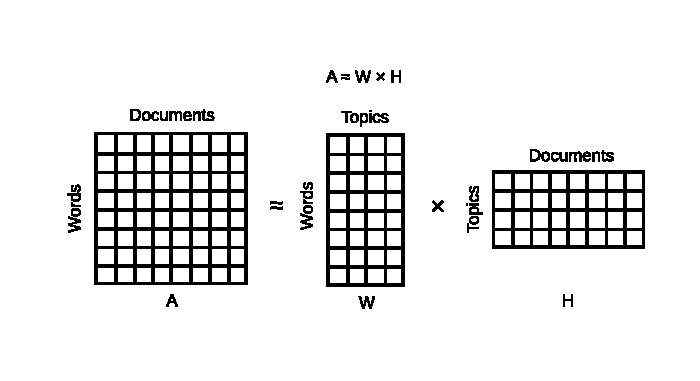
\includegraphics[width=0.75\textwidth]{figures/nmf.pdf}
    \caption{NMF decomposition}
    \label{fig:nmf}
\end{figure}

Non-negative Matrix Factorization is a group of algorithms whose objective is to minimize $F$ - the function which measures the error between the original matrix and the product of the two matrices. The most common algorithms for NMF typically involve iterative update rules that aim to minimize $F$, such as the Frobenius norm or the Kullback-Leibler (KL) divergence.

\subsection{Frobenius norm}

The goal in NMF using the Frobenius norm is to minimize the objective function \( F \), which is given by:

\[
    F = \| A - WH \|_F^2 = \sum_{i=1}^{n} \sum_{j=1}^{m} (A_{ij} - (WH)_{ij})^2
\]

where \( \| \cdot \|_F \) denotes the Frobenius norm. This objective function represents the sum of the squares of the element-wise differences between \( A \) and the product \( WH \).

The typical algorithm to minimize the Frobenius norm in NMF is an iterative process that involves:

\begin{enumerate}
    \item \textbf{Initialization:} Matrices \( W \) and \( H \) are initialized with non-negative values. This can be done randomly or based on some informed heuristic.
    \item \textbf{Iterative Update:} The matrices \( W \) and \( H \) are updated iteratively to reduce \( F \). The updates are performed using multiplicative rules that inherently maintain the non-negativity of \( W \) and \( H \). The update rules are as follows:
          \[
              W_{ai} \leftarrow W_{ai} \cdot \frac{(AH^\top)_{ai}}{(WHH^\top)_{ai}}
          \]
          \[
              H_{ib} \leftarrow H_{ib} \cdot \frac{(W^\top A)_{ib}}{(W^\top WH)_{ib}}
          \]
          where the indices \( a \) and \( b \) iterate over all rows and columns of \( W \) and \( H \), respectively.
    \item \textbf{Convergence:} The iteration continues until the change in \( F \) between successive iterations is less than a predetermined threshold, or a maximum number of iterations has been reached.
\end{enumerate}

While the Frobenius norm-based NMF is not convex over both \( W \) and \( H \) together, it is convex over each one individually when the other is held constant. Thus, each iteration is guaranteed to not increase \( F \), although the solution may converge to a local minimum rather than a global minimum.

\subsection{Kullback-Leibler}

Unlike the Frobenius norm which assesses the difference based on squared errors, the KL divergence is more suitable for data that is inherently probabilistic. The KL divergence for two matrices is defined as:

\[
    D(A || WH) = \sum_{i=1}^{n} \sum_{j=1}^{m} \left( A_{ij} \log\frac{A_{ij}}{(WH)_{ij}} - A_{ij} + (WH)_{ij} \right)
\]

where \( D(A || WH) \) represents the KL divergence between \( A \) and \( WH \), with the objective to minimize this divergence in NMF.

The iterative update rules for the matrices \( W \) and \( H \) that minimize the KL divergence are as follows:

\[
    W_{ai} \leftarrow W_{ai} \cdot \frac{(A \oslash (WH)H^\top)_{ai}}{\mathbf{1}H^\top_{ai}}
\]

\[
    H_{ib} \leftarrow H_{ib} \cdot \frac{(W^\top(A \oslash (WH)))_{ib}}{W^\top\mathbf{1}_{ib}}
\]

Here, \( \oslash \) denotes element-wise division, and \( \mathbf{1} \) is a matrix of ones that is used for normalization in the denominators.

Just like in the case of the Frobenius norm, the KL divergence-based NMF aims to iteratively update \( W \) and \( H \) until the decrease in \( D(A || WH) \) is below a certain threshold, signaling convergence. However, it is important to note that this optimization problem is non-convex, and the solution found may represent a local minimum.

\section{Top2Vec}
\label{sec:top2vec}
A limitation of LDA and NMF is that they disregard semantic relationships between words, thus neglecting context. As a result, text embedding techniques which capture context have become popular as an NLP technique.

\subsection{Embeddings}

In Top2Vec \cite{angelov_top2vec_2020}, the first step is to embed the documents into dense vector representations (embeddings) to capture the semantic meaning of the text. \Cref{fig:doc_word_embedding} \cite{angelov_top2vec_2020} illustrates the embeddings, where the purple dots represent words and the green dots represent documents. Words are closest to documents that contain them, and documents are closest to words that are most representative of their content.

\begin{figure}[h] % adjust placement if needed
    \centering
    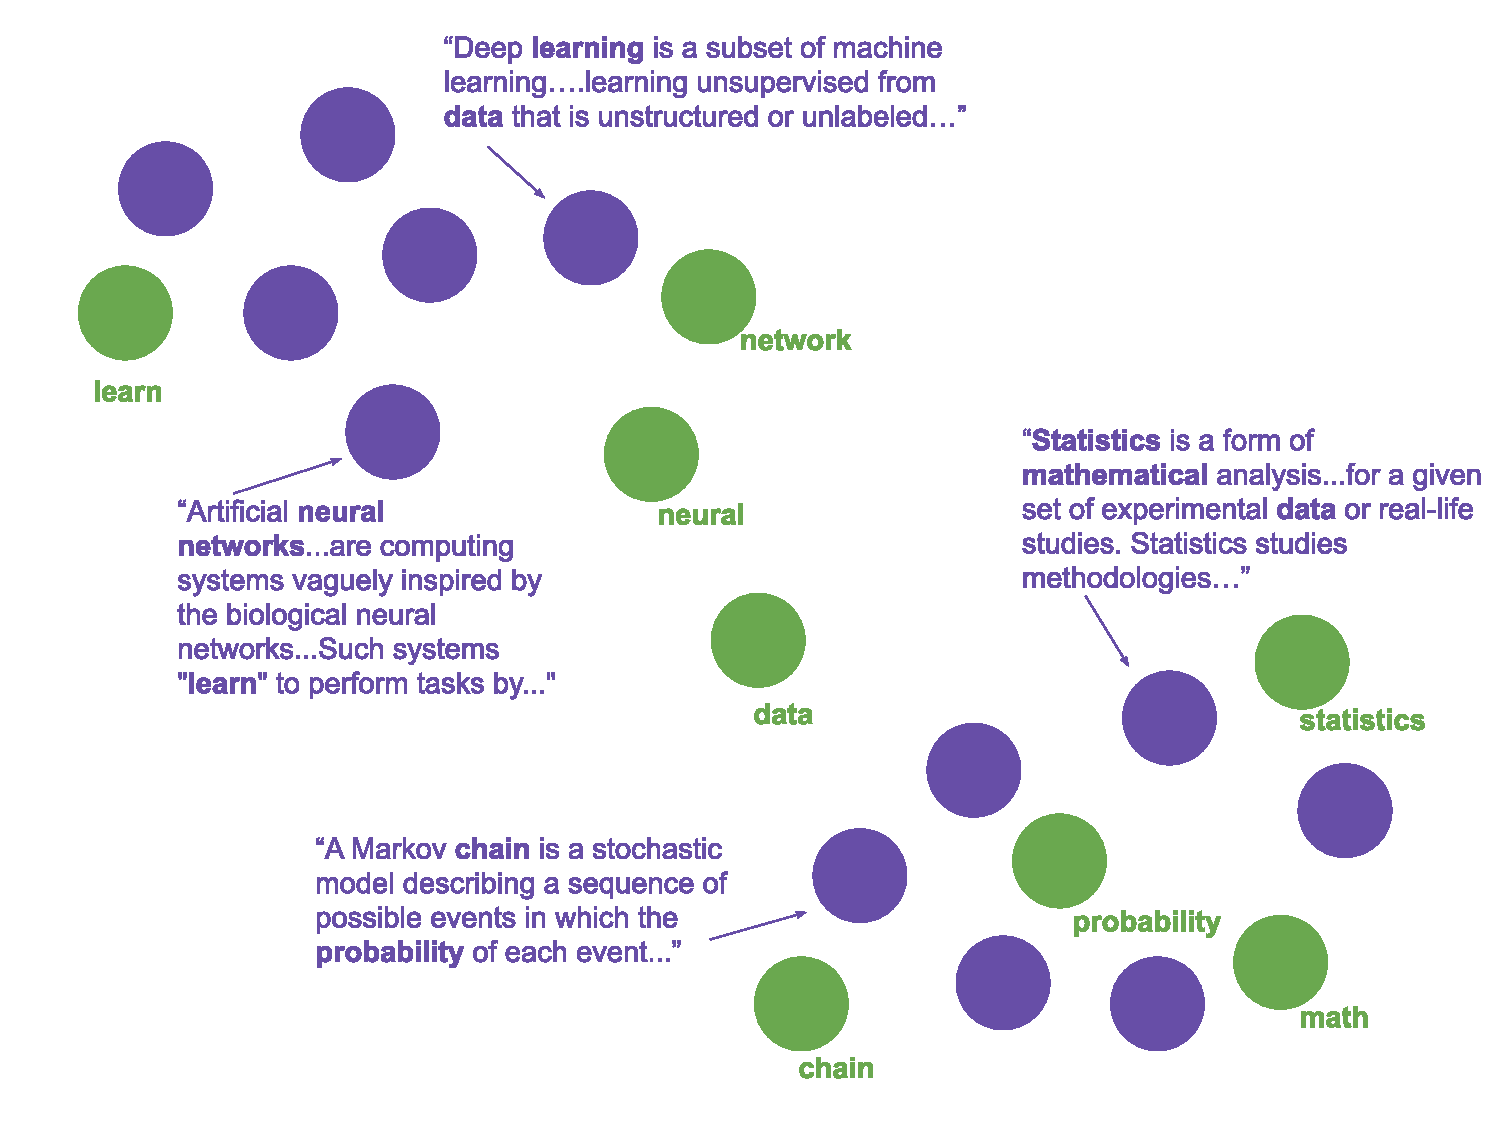
\includegraphics[width=0.65\textwidth]{figures/doc_word_embedding.pdf}
    \caption{Example of embeddings}
    \label{fig:doc_word_embedding}
\end{figure}

To learn the embeddings, Top2Vec utilizes Doc2Vec \cite{le_distributed_2014, rehurek_software_2010}, Universal Sentence Encoder \cite{cer_universal_2018}, or Sentence-BERT (SBERT) \cite{reimers_sentence-bert_2019}.

The original paper uses Doc2Vec's Distributed Bag of Words (DBOW) model, and even though it is simpler than Doc2Vec's Distributed Memory (DM) model, it is more efficient and has been shown to perform better in practice \cite{lau_empirical_2016}. DBOW essentially uses the document vector to predict words within a context window in the document.

Doc2Vec's DBOW is similar to Word2Vec's Skip-gram model (\cref{sec:word_embedding_topic_models}), which uses the context word to predict surrounding words in the context window. The difference is that DBOW switches the context word for the document vector to predict the surrounding words in the context window.

The process of learning the embeddings in Top2Vec can be summarized as follows:
\begin{enumerate}
    \item \textbf{Matrix Initialization}: The process initiates with the establishment of two matrices. The document matrix, denoted as $D_{c,d}$, encapsulates document vectors where $c$ represents the corpus's document count and $d$ the embedding dimensionality. Each row within $D_{c,d}$ represents a distinct document vector $\vec{d} \in \mathbb{R}^d$. Concurrently, the context word matrix $W'_{n,d}$, representing word vectors in analogous $d$-dimensional space for $n$ vocabulary words, may originate from pre-training, random initialization, or parallel learning processes.

    \item \textbf{Word Prediction Mechanism}: Contrary to relying on neighboring context words for prediction, the DBOW model employs the document vector for prediction. For every document $d$, each word's context vector $\vec{w_c}'$ within $d$ (sourced from $W'_{n,d}$) aids in inferring the document's vector $\vec{d}$ in $D_{c,d}$. This inference employs a softmax function, $\text{softmax}(\vec{w_c}' \cdot D_{c,d})$, generating a corpus-wide probability distribution reflecting each document's likelihood of generating the word.

    \item \textbf{Learning Process}: The learning process aims to optimize the document and word vectors to predict the document's constituent words. This optimization leverages backpropagation and stochastic gradient descent to modify both $D_{c,d}$ and $\vec{w_c}'$ from $W'_{n,d}$ to maximize the probability $P(\vec{d} | \vec{w})$ of correctly predicting the document given its words.

    \item \textbf{Embeddings}: Through optimization, embeddings emerge where documents gravitate towards the vectors of words they comprise, effectively "attracted" by these words. Consequently, semantically similar documents (sharing similar words) cluster, whereas dissimilar documents (sharing fewer words) diverge.
\end{enumerate}

\subsection{Number of topics}

In the embeddings, a dense area of documents can be interpreted as an area of highly similar documents. First, Uniform Manifold Approximation and Projection for Dimension Reduction (UMAP) \cite{mcinnes_umap_2020} is used to reduce the dimensionality of the document vectors. That is because the high-dimensional document vectors lead to the \textit{curse of dimensionality}, where the document vector sparsity makes it difficult to find dense clusters. Then, in order find the dense areas of documents in the embeddings, density-based clustering is used on the document vectors, specifically Hierarchical Density-Based Spatial Clustering of Applications with Noise (HDBSCAN) \cite{campello_density-based_2013, mcinnes_accelerated_2017, mcinnes_hdbscan_2017}. HDBSCAN assigns a label to each dense cluster of document vectors and assigns a noise label to all document vectors that are not in a dense cluster.


\subsection{Topic vectors}

Given labels for each cluster of dense documents in the embeddings, topic vectors can be calculated. The authors lay out multiple methods for calculating topic vectors, but discover that they perform similarly. The method that is used in the original paper is to calculate the centroid of the document vectors in each cluster. The centroid is the average of all the document vectors in the cluster. The centroid is calculated for each set of document vectors that belong do a dense cluster, generating a topic vector for each set. The number of dense areas found is the number of prominent topics identified in the corpus.

In the embeddings, every point represents a topic that is best described semantically by its nearest word vectors. Therefore, the word vectors that are closest to a topic vector are those that are most representative of it semantically. The distance of each word vector to the topic vector will indicate how semantically similar the word is to the topic. The words closest to the topic vector can be seen as the words that are most similar to all documents into the dense area, as the topic vector is the centroid of that area. These words can be used to summarize the common topic of the documents in the dense area.

\section{BERTopic}
\label{sec:bertopic}
Top2Vec simplifies the process of generating topics by clustering embeddings of words and documents. Inspired from Top2Vec, BERTopic \cite{grootendorst_bertopic_2022} is a state-of-the-art topic model that builds on top of the embeddings approach.

BERTopic generates representations of topics through a six-step process:

\begin{enumerate}
    \item Initially, it transforms each document into an embedding using a pre-trained language model.
    \item Before the clustering process, the dimensionality of these embeddings is reduced.
    \item Following this, the embeddings are clustered.
    \item Subsequently, a bag-of-words representation is generated for each cluster, containing the frequency of every word.
    \item Next, topic representations are derived from these clusters using a specialized class-based version of TF-IDF.
    \item The final step optionally fine-tunes these topic representations. Each of these steps is modular, allowing for the use of different techniques at each stage.
\end{enumerate}

While these steps are the default, BERTopic offers a degree of modularity. Each step in the process is relatively independent from the others. For instance, the bag-of-words step does not depend on the specific embedding model used for document embeddings, which provides flexibility in how the bag-of-words representation is calculated.

As a result, BERTopic is highly modular, maintaining its ability to generate topics across different submodels. This means that BERTopic effectively allows for the construction of customized topic models, appropriate for the specific use case. Additionally, the modularity of BERTopic ensures that it can be easily adapted to incorporate new advancements in the field of NLP, since each component can be changed independently from the others. \Cref{fig:modularity_modified} (inspired by \cite{grootendorst_algorithm_nodate}) illustrates the six steps of BERTopic, presented from bottom to top. It highlights the possibility of employing various techniques at each step of the process. For example, one could choose between SBERT or spaCy for document embedding, UMAP \cite{mcinnes_umap_2020} or PCA \cite{abdi_principal_2010} for dimensionality reduction, and GPT or KeyBERT \cite{grootendorst_maartengrkeybert_2024} for the fine-tuning phase.

\begin{figure}[h] % adjust placement if needed
    \centering
    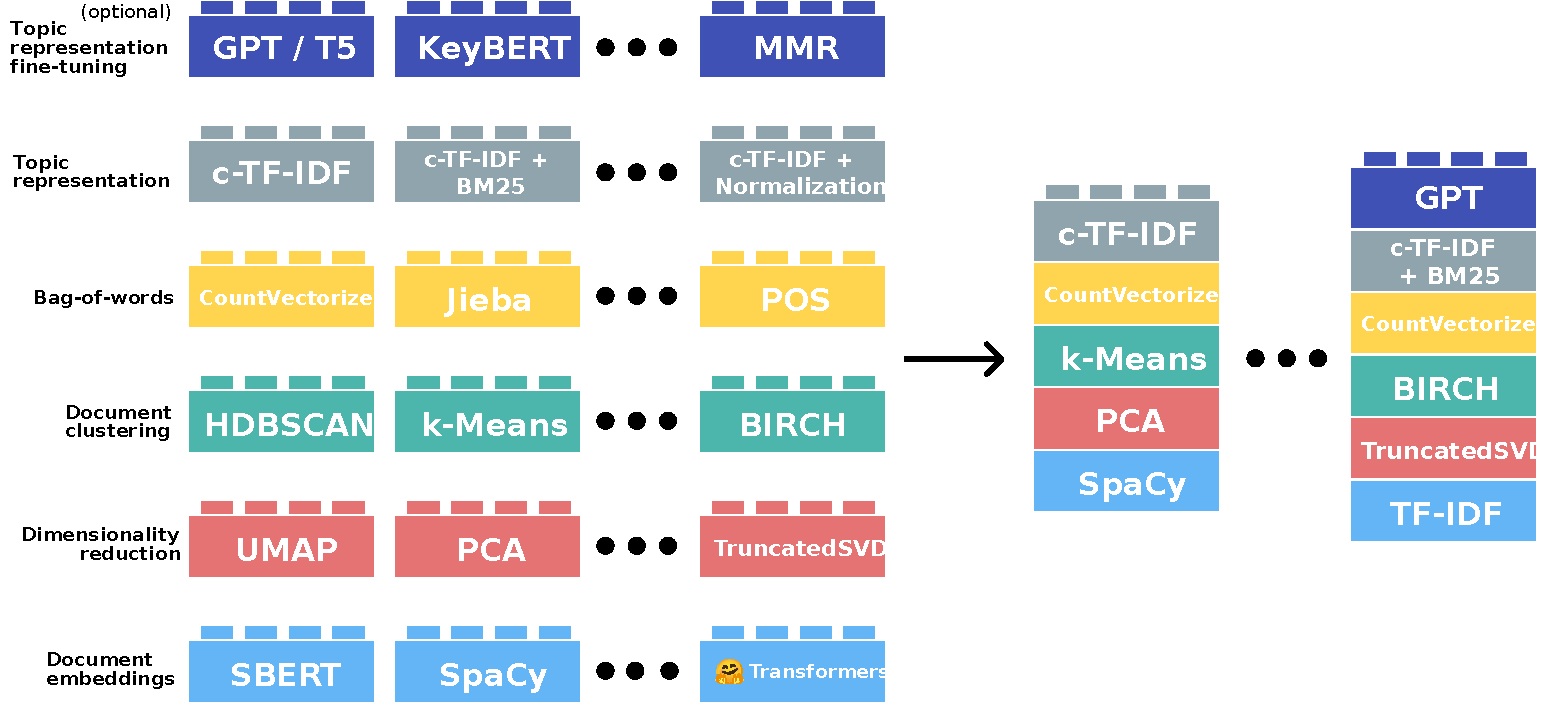
\includegraphics[width=\textwidth]{figures/modularity_modified.pdf}
    \caption{BERTopic modularity and steps (from bottom to top)}
    \label{fig:modularity_modified}
\end{figure}

\subsection{Document embeddings}

In BERTopic, documents are transformed into embeddings to create vector space representations for semantic comparison. It is based on the idea that documents sharing the same topic will have similar semantics. For this embedding step, by default BERTopic utilizes the SBERT framework \cite{reimers_sentence-bert_2019}. SBERT is a modification of the popular Bidirectional Encoder Representations from Transformer (BERT) model (\cref{sec:transformer_based_models}), and enables the conversion of sentences and paragraphs into dense vector representations by employing pre-trained language models. This achieves top performance on several sentence embedding tasks \cite{reimers_making_2020}. The embeddings are mainly used for clustering documents with semantic similarities rather than directly for topic generation.

The base Transformer architecture is presented in \cref{fig:transformer} \cite{vaswani_attention_2017}. It uses a unidirectional multi-head self-attention mechanism to capture dependencies between words in a sentence. Unidirectional means that the attention mechanism only looks at previous words in the sentence, which can be a limitation. The model consists of a stacked encoder-decoder architecture, where the encoder processes the input sequence, and the decoder generates the output sequence. The encoder is composed of a stack of identical layers, each containing two sub-layers: a multi-head self-attention mechanism and a feed-forward neural network. The decoder is also composed of a stack of identical layers, each containing three sub-layers: a multi-head self-attention mechanism, a multi-head attention mechanism over the encoder's output, and a feed-forward neural network. The self-attention mechanism allows the model to weigh the importance of each word in the sentence when generating the embeddings.

\begin{figure}[h]
    \centering
    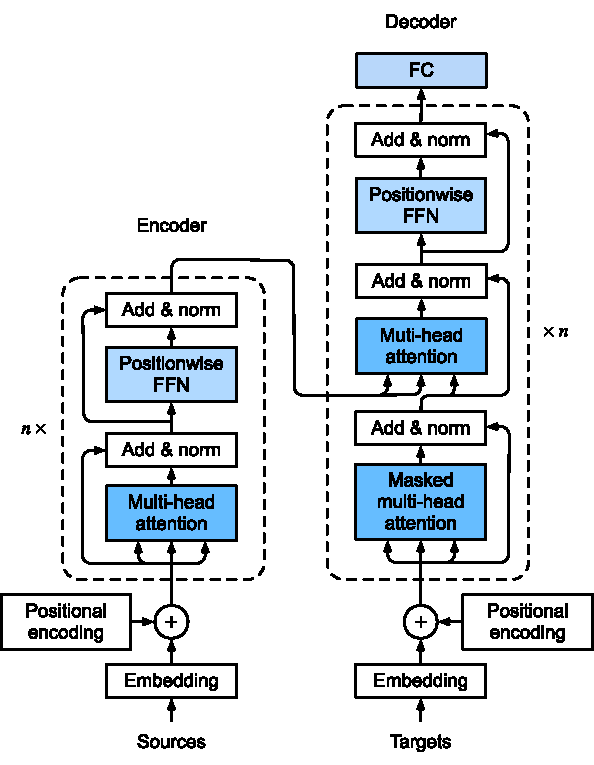
\includegraphics[width=0.5\textwidth]{figures/transformer.pdf}
    \caption{Transformer architecture}
    \label{fig:transformer}
\end{figure}

BERT, in contrast, is a bidirectional model that captures dependencies between words in both directions (\cref{fig:bert}, \cref{fig:gpt}, \cref{fig:bert_detailed}) \cite{vaswani_attention_2017, devlin_bert_2019}. It achieves this by leveraging a \textit{masked language model (MLM)} objective, where the model is trained to predict masked words within a sentence. Pre-trained on a large corpus of text, BERT’s embeddings can be fine-tuned for various downstream tasks, such as sentence classification or question answering. However, tasks relevant to topic modeling, such as semantic similarity, are computationally expensive due to BERT's cross-encoder architecture. In a cross-encoder, pairs of sentences are passed through the transformer network together, and the target value is predicted. For example, in a collection of \( n = 10,000 \) sentences, finding the most similar pair using BERT would require \( n \times (n-1) / 2 = 49,995,000 \) inference computations \cite{reimers_sentence-bert_2019}.

\begin{figure}[h]
    \centering
    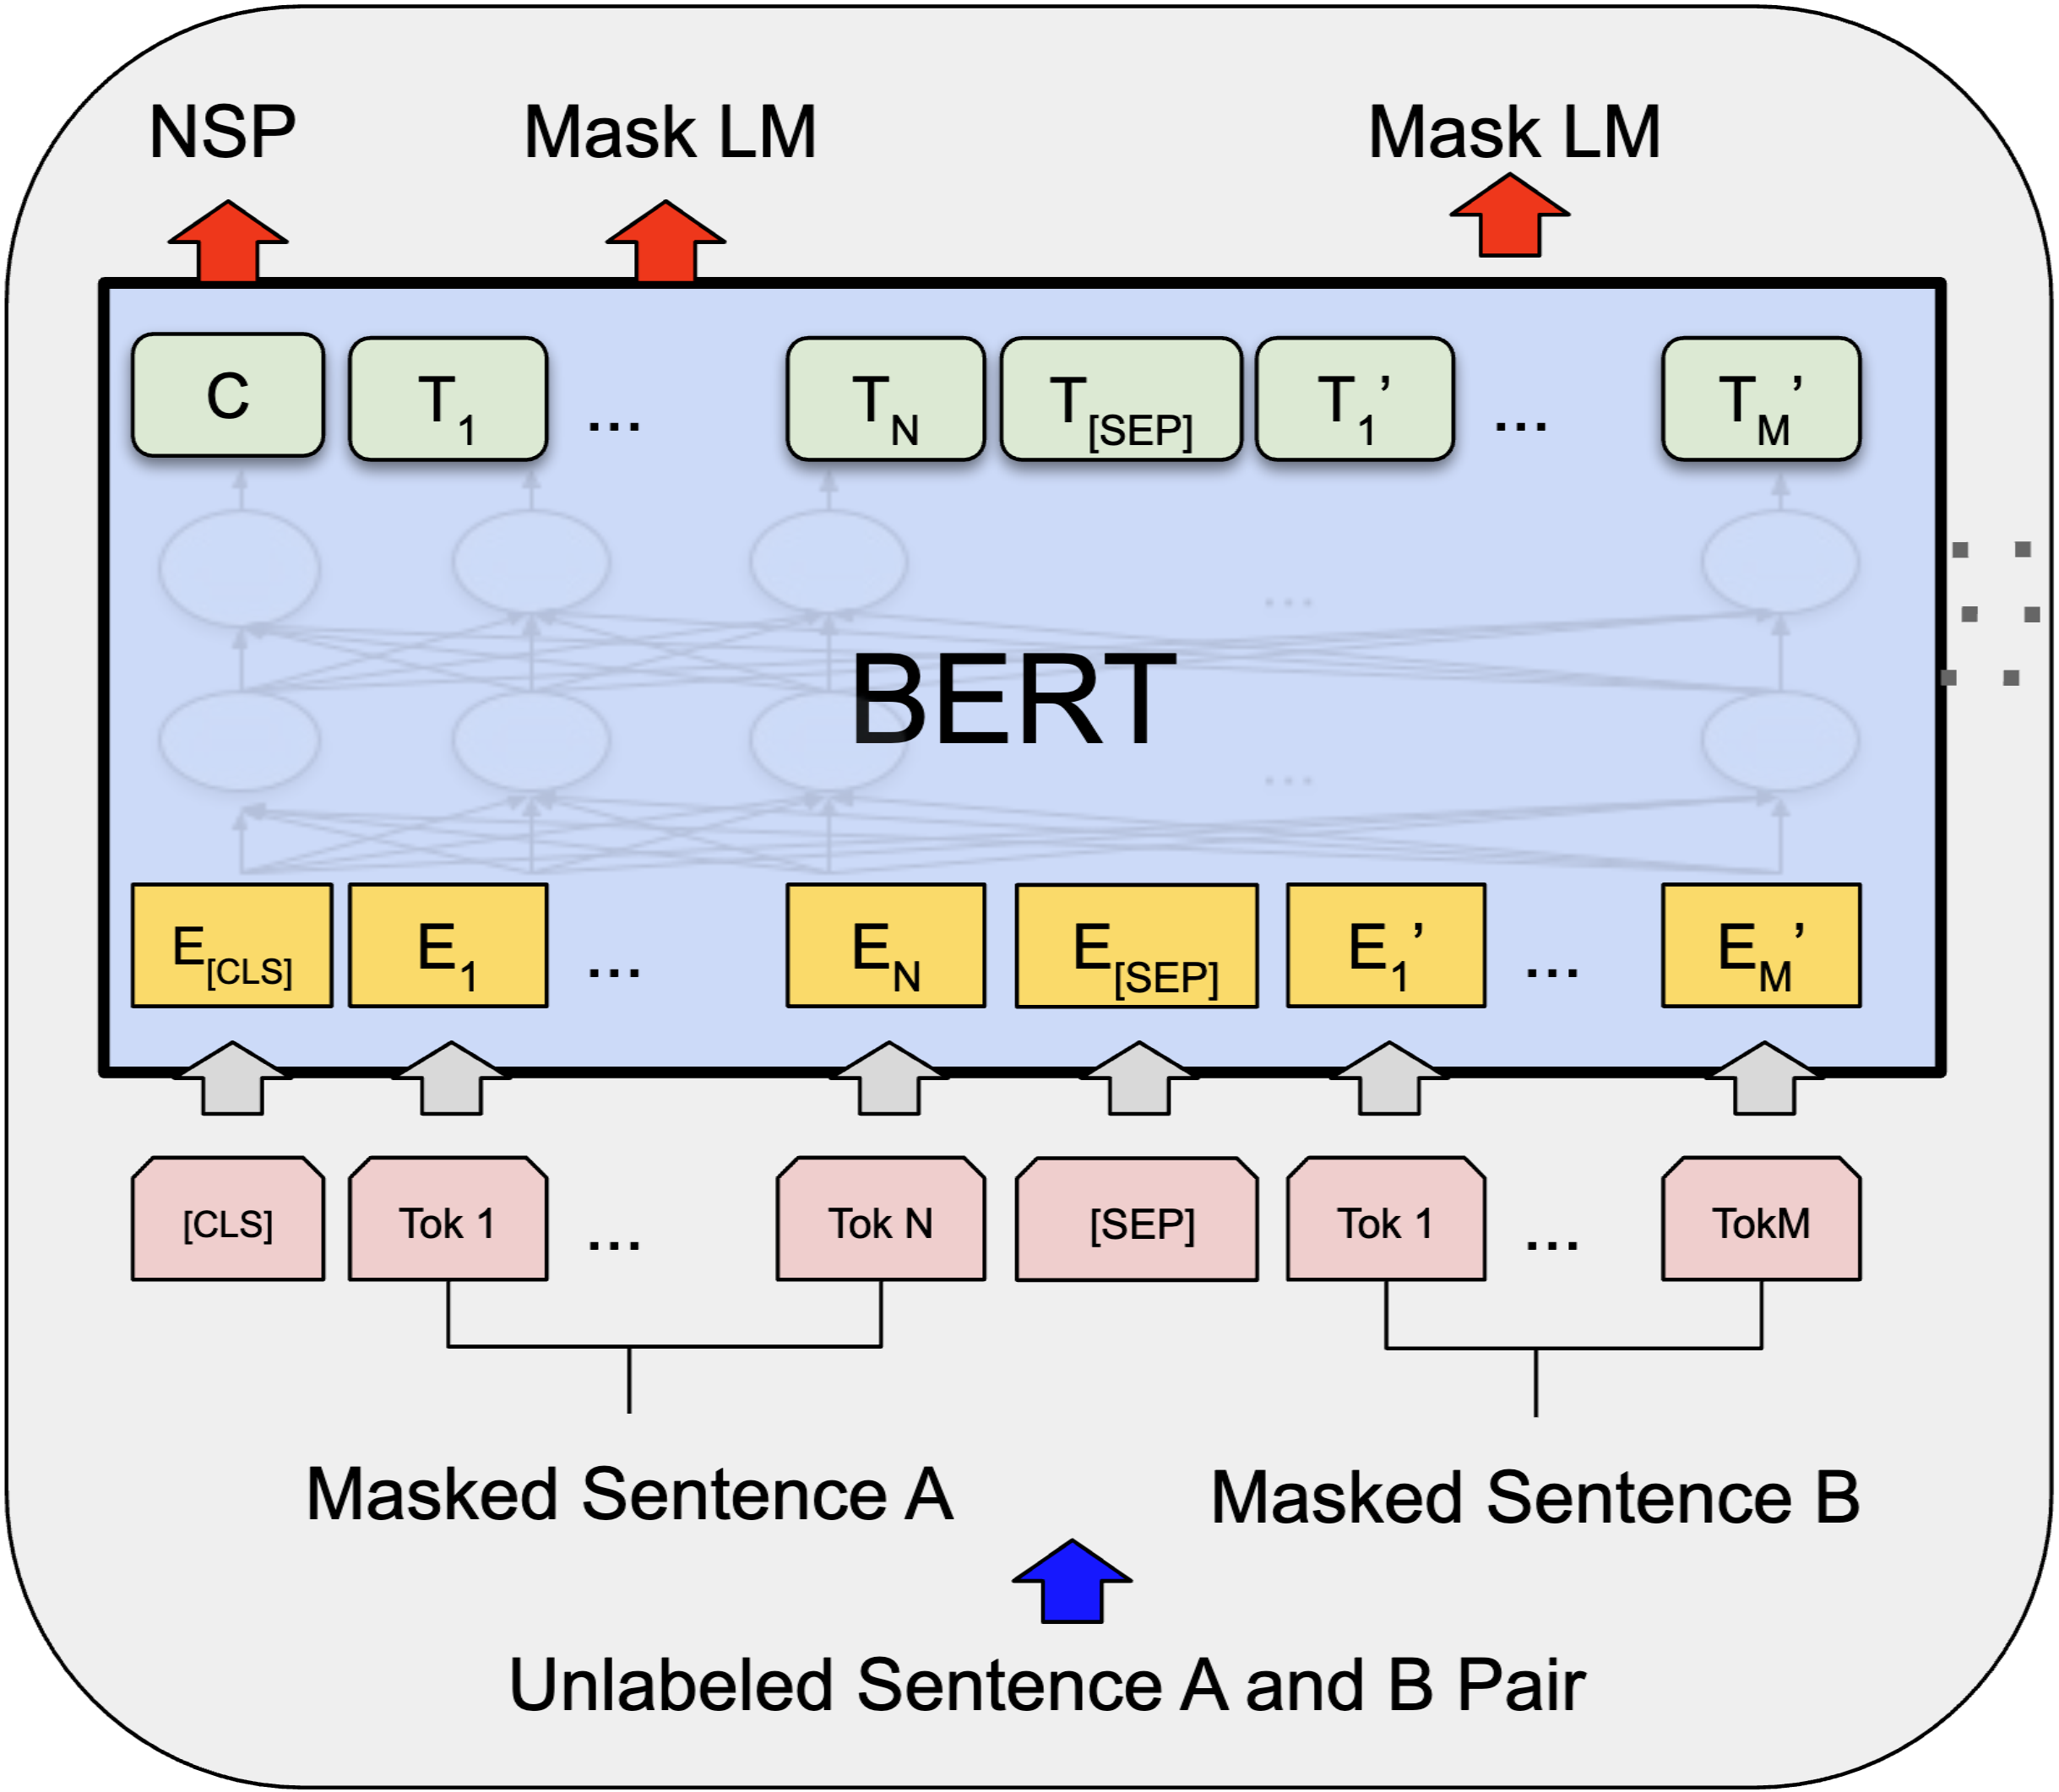
\includegraphics[width=0.5\textwidth]{figures/bert_detailed.png}
    \caption{BERT architecture}
    \label{fig:bert_detailed}
\end{figure}

\begin{figure}[h]
    \centering
    \begin{minipage}[b]{0.40\textwidth}
        \centering
        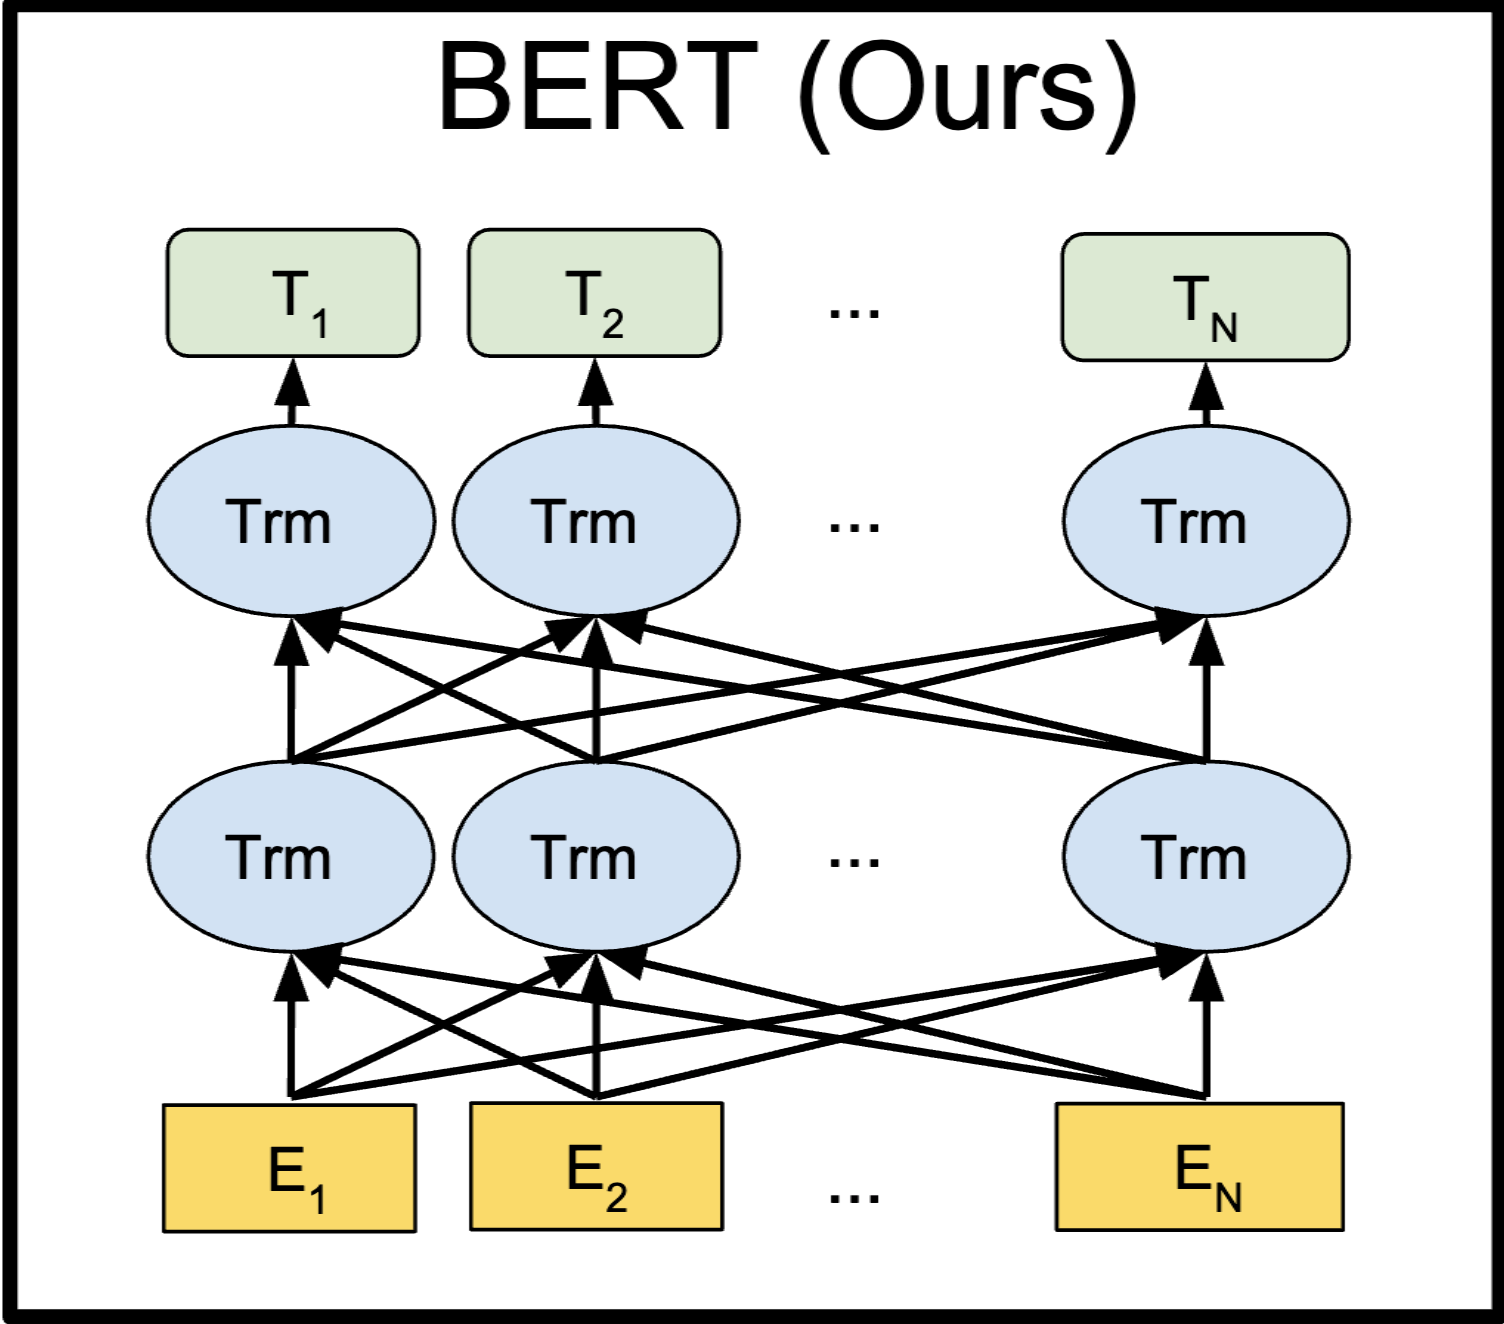
\includegraphics[width=\textwidth]{figures/bert.png}
        \caption{BERT bidirectional architecture}
        \label{fig:bert}
    \end{minipage}
    \hfill
    \begin{minipage}[b]{0.39\textwidth}
        \centering
        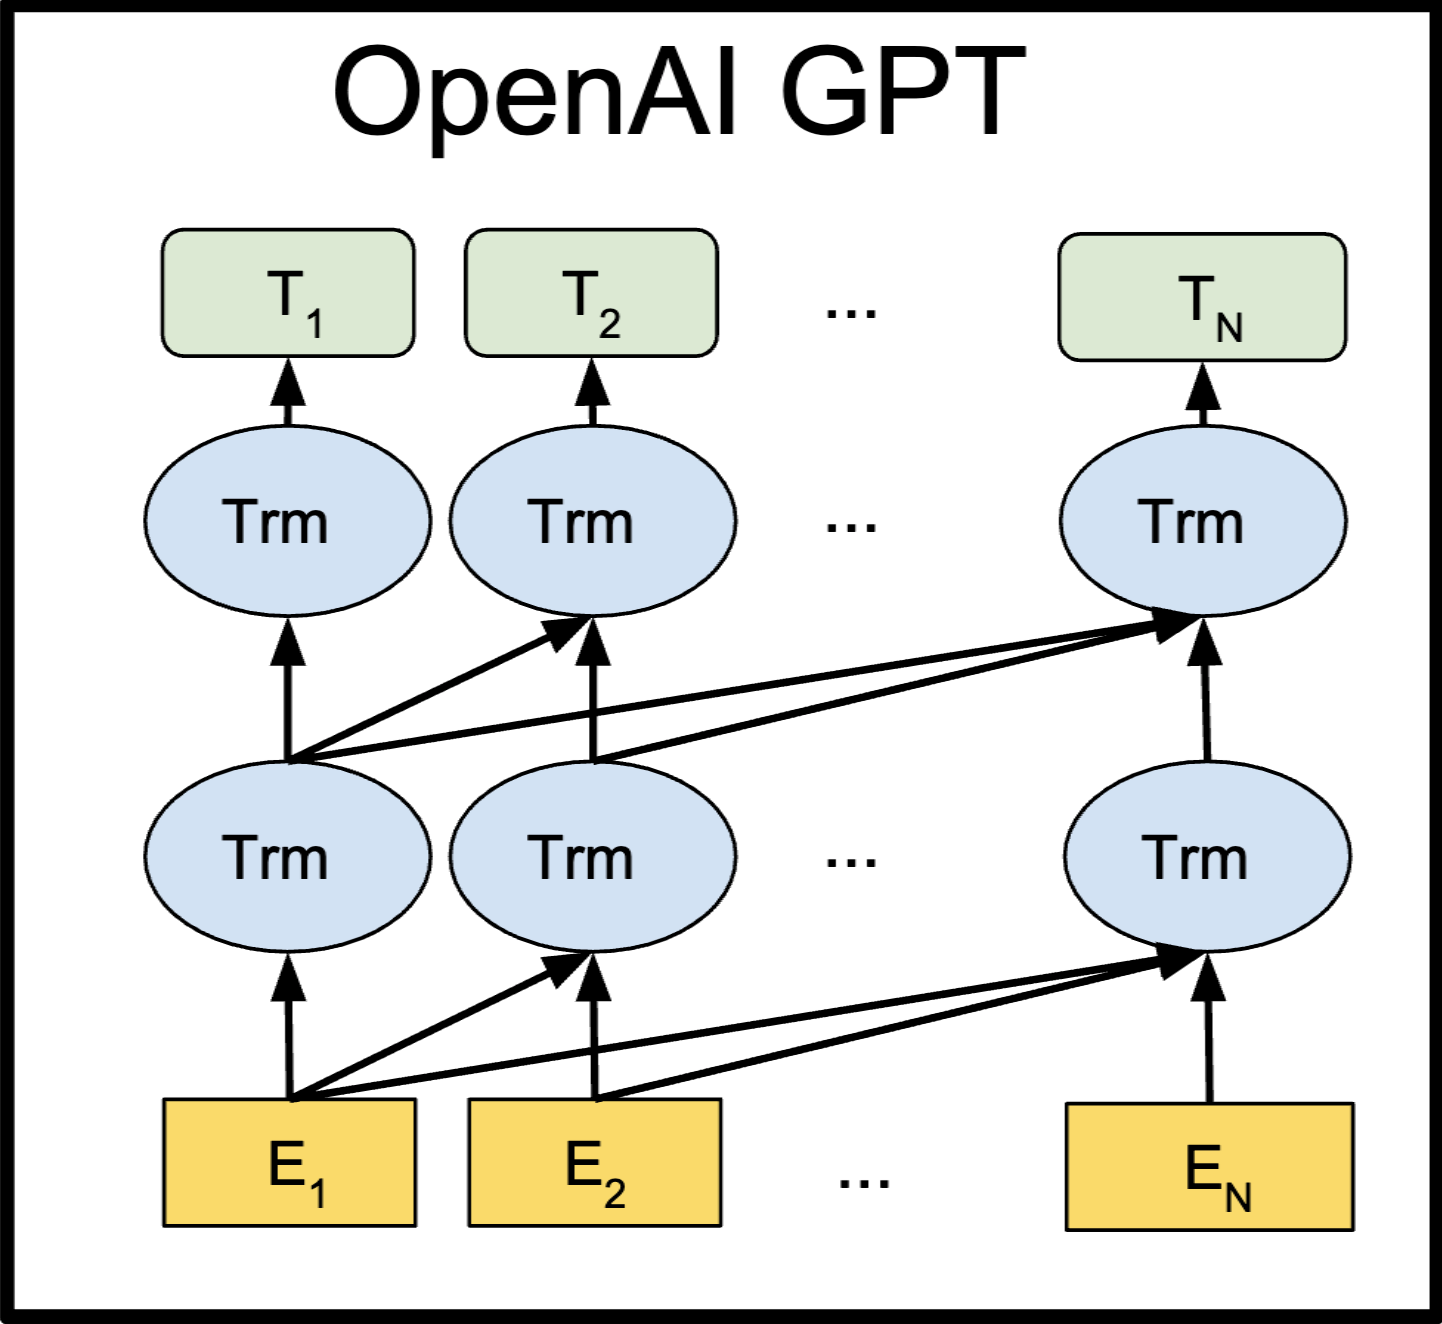
\includegraphics[width=\textwidth]{figures/openai.png}
        \caption{OpenAI GPT unidirectional architecture}
        \label{fig:gpt}
    \end{minipage}
\end{figure}

SBERT addresses this issue by incorporating a Siamese network architecture with a bi-encoder setup, where two identical BERT models share the same weights (\cref{fig:bi_vs_cross}). In SBERT, each sentence is processed independently, and the embeddings are computed separately. As a result, for \( n = 10,000 \) sentences, only 10,000 inference computations are needed. Once the embeddings are generated, similarity can be easily calculated, as it is a computationally efficient operation.

\begin{figure}[h]
    \centering
    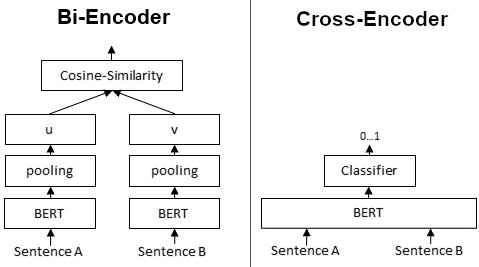
\includegraphics[width=0.6\textwidth]{figures/bi_vs_cross.png}
    \caption{Transformer architecture}
    \label{fig:bi_vs_cross}
\end{figure}

GPT \cite{radford_improving_nodate, radford_language_nodate, brown_language_2020}, BERT \cite{devlin_bert_2019}, T5 \cite{raffel_exploring_2020} and other similar models based on transformers are called large language models (LLMs). They are pre-trained on large corpora of text data and fine-tuned for specific tasks. LLMs have been shown to achieve state-of-the-art performance on a wide range of NLP tasks, including text classification, question answering, and language translation. However, the computational cost of training and fine-tuning LLMs is high, and they require large amounts of data to achieve good performance. In addition, LLMs are often criticized for their lack of interpretability, as the internal workings of the model are complex and difficult to understand.

BERTopic can use any embedding technique or architecture, provided the language model used for generating document embeddings is fine-tuned for semantic similarity. Hence, the quality of BERTopic's clustering improves as more advanced language models are developed, allowing BERTopic to evolve alongside advancements in embedding techniques. This proves particularly useful in the context of topic modeling, since the quality of the embeddings directly influences the quality of the topics generated.

The Massive Text Embedding Benchmark (MTEB) \cite{muennighoff_mteb_2023} is a benchmark that evaluates the performance of various embedding models on a wide range of tasks. It provides a comprehensive comparison of the performance of different embedding models, including SBERT, RoBERTa \cite{liu_roberta_2019}, and BERT. By leveraging MTEB, the user can select the most suitable embedding model for their specific use case.

\subsection{Dimensionality reduction}

As the dimensionality of data (embeddings) increases, the distance to the nearest data point tends to become similar to the distance to the farthest data point \cite{aggarwal_surprising_2001, beyer_when_1999}. This phenomenon implies that in high-dimensional spaces, the notion of spatial locality becomes unclear, and distances between points become increasingly small. While several clustering methods have been developed to address this \textit{curse of dimensionality} \cite{pandove_systematic_2018, steinbach_challenges_2004}, a simpler strategy involves reducing the dimensionality of embeddings. Although PCA \cite{abdi_principal_2010} and t-SNE \cite{van_der_maaten_visualizing_2008} are popular dimensionality reduction techniques, UMAP has been found to better preserve the local and global characteristics of high-dimensional data in its lower-dimensional representations \cite{mcinnes_umap_2020}.

UMAP is a non-linear dimensionality reduction technique that is rooted in manifold learning and is mathematically grounded in topological data analysis. More specifically, UMAP seeks to approximate a high-dimensional manifold by constructing a weighted k-nearest neighbor (k-NN) graph and then optimizing a low-dimensional layout of this graph.

The theory behind UMAP is more mathematically complex, but the algorithm can be summarized as follows:

1. \textbf{Constructing the k-NN Graph}:\\
The initial phase of UMAP involves constructing a k-nearest neighbor graph from the high-dimensional data. In this step, for each data point, the algorithm identifies its nearest neighbors based on a distance metric (such as Euclidean distance). The choice of $k$ determines the number of neighbors to consider, and this influences the local structure captured by the graph. Importantly, UMAP assumes that the data points are uniformly distributed on the underlying manifold, and it computes a local distance metric for each point using \textit{Riemannian geometry}. This local metric is based on the distance to the $k$-th nearest neighbor, creating a unique distance function for each point.

2. \textbf{Fuzzy Simplicial Complex Representation}:\\
Once the k-NN graph is built, UMAP constructs a fuzzy simplicial complex. This is a crucial step rooted in topological data analysis. Instead of a binary decision about whether or not a point belongs to a neighborhood, UMAP assigns fuzzy membership values to reflect the probability of points being connected. This fuzzy approach smooths out the local connectivity of the manifold. The fuzzy simplicial set is built by combining local fuzzy simplicial sets of each point, using a probabilistic union operation to merge the connections between points. This union operation involves combining the fuzzy memberships of edges (1-simplices) between points, which can be expressed mathematically as $w(e) = a + b - ab$, where $a$ and $b$ are the fuzzy membership probabilities for the edge in each direction, and $w(e)$ is the resulting combined weight.

3. \textbf{Low-Dimensional Embedding Optimization}:\\
After constructing the fuzzy topological representation, UMAP seeks to optimize a low-dimensional embedding that preserves the topological structure of the original data. This process can be viewed as a \textit{graph layout problem}. UMAP minimizes the cross-entropy between the fuzzy topological structures of the high-dimensional data and the low-dimensional embedding. The cross-entropy loss is given by:

\[
    \sum_{e \in E} w_h(e) \log \left( \frac{w_h(e)}{w_l(e)} \right) + (1 - w_h(e)) \log \left( \frac{1 - w_h(e)}{1 - w_l(e)} \right)
\]

Here, $w_h(e)$ and $w_l(e)$ represent the fuzzy membership weights of the edge $e$ in the high-dimensional and low-dimensional spaces, respectively. The first term represents an \textit{attractive force}, pulling points that are close in the high-dimensional space to be close in the low-dimensional space. The second term represents a \textit{repulsive force}, pushing points that are distant in the high-dimensional space to remain distant in the low-dimensional space.

4. \textbf{Use of Negative Sampling}:\\
To further optimize the computational efficiency of the embedding process, UMAP uses the \textit{negative sampling trick}, similar to methods employed in algorithms like \textit{word2vec} and \textit{LargeVis}. Instead of computing the cross-entropy over all possible pairs of points, UMAP samples a subset of non-neighboring points (negative samples) to approximate the repulsive forces. This reduces the computational complexity, making the algorithm scalable to large datasets.

5. \textbf{Stochastic Gradient Descent (SGD) Optimization}:\\
The optimization of the low-dimensional embedding is performed using \textit{stochastic gradient descent (SGD)}. The final objective function is designed to be differentiable, allowing for efficient gradient-based optimization. UMAP uses a smooth approximation for the membership strength function in the low-dimensional space, typically of the form $\frac{1}{1 + a x^{2b}}$, where $a$ and $b$ are curve parameters selected to best approximate the fuzzy memberships in the low-dimensional space. The optimization process iteratively adjusts the positions of points in the low-dimensional space until the cross-entropy loss is minimized.

6. \textbf{Initialization with Spectral Embedding}:\\
To speed up convergence, UMAP often initializes the low-dimensional embedding using \textit{spectral embedding techniques}. This involves computing the eigenvectors of the graph Laplacian, which provides an initial guess for the positions of the points in the low-dimensional space. The spectral embedding serves as a good starting point for the SGD optimization.

By combining these steps, UMAP produces a low-dimensional embedding that preserves both the local and global structure of the high-dimensional data.

\subsection{Document clustering}

The reduced embeddings are clustered using a clustering model/algorithm. A popular choice is HDBSCAN (Hierarchical Density-Based Spatial Clustering of Applications with Noise) \cite{campello_density-based_2013, campello_hierarchical_2015, mcinnes_accelerated_2017, mcinnes_hdbscan_2017}. HDBSCAN is built on top of DBSCAN \cite{ester_density-based_nodate} and is designed to identify clusters of various densities by transforming DBSCAN into a hierarchical clustering algorithm. It employs a soft-clustering approach, which allows for the treatment of noise as outliers. Traditional clustering assigns each point in a dataset to a cluster, which is a hard assignment without mixed memberships. Conversely, in soft clustering, points are not assigned a cluster label, but are instead assigned a vector of probabilities. This allows points to potentially be a mix of clusters. Soft clustering is particularly useful in topic modeling, as documents can belong to multiple topics.

Furthermore, \citet{allaoui_considerably_2020} showed that the performance of well-known clustering algorithms, including k-Means and HDBSCAN, can be significantly improved by reducing the dimensionality of high-dimensional embeddings with UMAP, in terms of both clustering accuracy and computational time.

HDBSCAN combines hierarchical clustering with density-based clustering. HDBSCAN's algorithm can be summarized as follows:

1. \textbf{Core Distance Calculation}: \\
The first step in HDBSCAN is similar to DBSCAN, but instead of using a fixed distance threshold ($\epsilon$), HDBSCAN calculates the \textit{core distance} for each point in the dataset. The core distance of a point $x_p$ with respect to a parameter \texttt{min\_samples} is defined as the distance to its \texttt{min\_samples}-th nearest neighbor:
\[
    d_{\text{core}}(x_p) = d(x_p, \text{min\_samples-th nearest neighbor}).
\]
This core distance acts as a local density estimate, and each point must have at least \texttt{min\_samples} points within its core distance to be considered a core point.

2. \textbf{Mutual Reachability Distance}: \\
To account for varying densities in the dataset, HDBSCAN uses the \textit{mutual reachability distance} between two points, $x_p$ and $x_q$. This is defined as the maximum of their core distances and the direct distance between them:
\[
    d_{\text{mreach}}(x_p, x_q) = \max \left( d_{\text{core}}(x_p), d_{\text{core}}(x_q), d(x_p, x_q) \right).
\]
This distance ensures that points in lower-density regions are only connected if they are sufficiently close to higher-density points.

3. \textbf{Constructing the Mutual Reachability Graph}: \\
Using the mutual reachability distance, HDBSCAN constructs a \textit{complete graph} where each data point is a vertex, and the weight of each edge between points $x_p$ and $x_q$ is given by $d_{\text{mreach}}(x_p, x_q)$. This graph is then used to create a \textit{minimum spanning tree} (MST), which forms the basis for the hierarchical structure of the clusters.

4. \textbf{Minimum Spanning Tree (MST) Construction}: \\
The next step is to construct the MST of the mutual reachability graph. This is done by connecting points in a way that minimizes the total edge weight while ensuring all points are connected. The MST provides a hierarchical structure where clusters can be formed by progressively cutting edges at increasing mutual reachability distances.

5. \textbf{Hierarchy of Clusters}: \\
As edges are removed from the MST in increasing order of mutual reachability distance, clusters start to form. Clusters in HDBSCAN are represented as connected components of the graph after removing edges. This process forms a \textit{hierarchical} clustering structure, where each cluster can potentially be split into subclusters at different distance thresholds.

6. \textbf{Cluster Stability and Excess of Mass}: \\
To extract the most significant clusters from the hierarchy, HDBSCAN measures the \textit{stability} of each cluster. Stability is a measure of how long a cluster persists as the mutual reachability distance increases. Formally, the stability of a cluster $C_i$ is defined as the relative excess of mass \cite{campello_density-based_2013}, which measures the area under the curve of the density function as the cluster shrinks:
\[
    S(C_i) = \sum_{x_j \in C_i} \left( \frac{1}{\epsilon_{\text{min}}(x_j, C_i)} - \frac{1}{\epsilon_{\text{max}}(C_i)} \right),
\]
where $\epsilon_{\text{min}}(x_j, C_i)$ is the minimum mutual reachability distance at which point $x_j$ is part of cluster $C_i$, and $\epsilon_{\text{max}}(C_i)$ is the distance at which $C_i$ either splits or disappears.

7. \textbf{Extracting the Optimal Flat Partition}: \\
Once the hierarchy of clusters is formed, HDBSCAN uses an optimization algorithm to extract the most significant flat partition of clusters. This selection is based on maximizing the sum of the stabilities of the clusters while ensuring that no nested clusters are selected simultaneously. The optimization problem can be formulated as:
\[
    \max \sum_{i=2}^{\kappa} \delta_i S(C_i), \quad \text{subject to } \sum_{j \in I_h} \delta_j = 1, \forall h \in L,
\]
where $\delta_i \in \{0, 1\}$ indicates whether cluster $C_i$ is included, $L$ is the set of leaf clusters, and $I_h$ is the set of all clusters on the path from leaf cluster $C_h$ to the root.

8. \textbf{Outlier Detection}: \\
Points that do not belong to any cluster are labeled as \textit{noise} or \textit{outliers}. These points either do not meet the density requirements to be considered part of a cluster or are isolated early in the hierarchical process. HDBSCAN is robust in handling noise, as it naturally separates outliers from dense regions of data.

9. \textbf{Soft Clustering with Probabilities}: \\
HDBSCAN also supports a \textit{soft clustering} mode, where instead of assigning a hard cluster label to each point, the algorithm calculates a \textit{membership probability} for each point to belong to a cluster. This is particularly useful in applications like topic modeling, where a document may belong to multiple topics. The membership probability $p(x_j \in C_i)$ for a point $x_j$ to cluster $C_i$ is derived from the distance and density estimates, allowing for more flexible cluster assignments.

\subsection{Bag-of-words}
\label{sec:bag_of_words}

Before creating topic representations in BERTopic, it is necessary to select a technique that supports the algorithm's modular nature, and does not make assumptions about the data. When using HDBSCAN, we assume that clusters may vary in density and shape, indicating that techniques based on centroid models may not be suitable. The desired method should ideally make minimal assumptions about the cluster structures.

The process begins by combining all documents within a cluster into a single document, which then represents the entire cluster. Subsequently, the frequency of each word within this single document is counted, resulting in a bag-of-words representation that reflects the word frequencies at the cluster level rather than the individual document level. The adoption of a bag-of-words approach ensures that no assumptions are made about the density and shape of the clusters.

There are various approaches to constructing a bag-of-words representation, facilitated by the use of \texttt{CountVectorizer}. \texttt{CountVectorizer} allows us to control the number of tokens in each topic representation. For instance, single words like \textit{game} or \textit{team} may appear in a topic, but it can also be useful to include multi-word phrases, such as \textit{hockey league}, which consist of two tokens. Additionally, some topics might include stop words, such as \textit{he} or \textit{the}, which are generally undesirable in topic representations as they provide little meaningful information. Removing these stop words is typically preferred to improve the quality of the topics.

To illustrate how topic representations can be constructed using a bag-of-words approach, let's consider an example where we have clustered documents related to sports. After applying HDBSCAN and merging the documents within each cluster into a single document, we can create a topic representation by counting the frequency of words and phrases within the merged document.

\cref{tab:hockey_cluster} shows a bag-of-words representation for a cluster related to hockey. The table includes both single words and multi-word phrases, and stop words have been removed to improve the quality of the representation.


\begin{table}[h]
    \centering
    \begin{tabular}{|c|c|}
        \hline
        \textbf{Word/Phrase} & \textbf{Frequency} \\
        \hline
        hockey               & 45                 \\
        league               & 32                 \\
        game                 & 28                 \\
        team                 & 27                 \\
        ice                  & 25                 \\
        hockey league        & 20                 \\
        playoff              & 18                 \\
        goals                & 15                 \\
        players              & 14                 \\
        national team        & 12                 \\
        championship         & 10                 \\
        tournament           & 9                  \\
        world cup            & 8                  \\
        goalie               & 7                  \\
        penalty              & 6                  \\
        \hline
    \end{tabular}
    \caption{Example Bag-of-Words representation for a hockey-related cluster}
    \label{tab:hockey_cluster}
\end{table}

\subsection{Topic representation}
\label{sec:topic_representation}
From the generated bag-of-words representation, our goal is to identify what distinguishes one cluster from another. Specifically, we want to determine which words are characteristic of a particular cluster (e.g., cluster 1) but less common in other clusters. To achieve this, we need to modify the traditional TF-IDF such that it operates at the cluster level, treating clusters as topics instead of individual documents.

The classic TF-IDF \cite{joachims_probabilistic_1997} method combines term frequency and inverse document frequency to calculate a weight $W_{t,d}$ for term $t$ in document $d$ as follows:

\[ W_{t,d} = tf_{t,d} \cdot \log\left(\frac{N}{df_t}\right) \]

Here, term frequency $tf_{t,d}$ represents the frequency of term $t$ in document $d$, and inverse document frequency measures $t$'s importance across documents, calculated by the logarithm of the ratio of the total number of documents $N$ to the number of documents containing $t$.


BERTopic extends the TF-IDF concept to clusters of documents by introducing class-based TF-IDF (c-TF-IDF). In this approach, documents within a cluster are concatenated into a single document, and the TF-IDF formula is modified for cluster-level representation:

\[ W_{t,c} = tf_{t,c} \cdot \log\left(1 + \frac{A}{tf_t}\right) \]

In this formula, term frequency $tf_{t,c}$ now models the frequency of term $t$ within a cluster $c$, treated as a single document. The inverse document frequency is substituted with an inverse class frequency, which assesses the term's importance to a cluster. This is calculated by the logarithm of the average number of words per cluster $A$ divided by the term's frequency $tf_t$ across all clusters, with $1$ added inside the logarithm to ensure positive values. This adaptation of TF-IDF to clusters allows us to model the importance of words in clusters instead of individual documents. Furthermore, by iteratively merging c-TF-IDF representations of less prevalent topics with their closest topics, the total number of topics can be reduced to meet a predefined threshold.

To illustrate this, consider the hockey-related cluster. Table \ref{tab:ctfidf_hockey} shows an example of how c-TF-IDF weights are calculated for several terms. As we can see from the table, terms like \textit{hockey}, \textit{ice}, and \textit{playoff} receive high c-TF-IDF weights because they are frequent in the hockey cluster but less common in other clusters. Conversely, terms such as \textit{game} and \textit{team}, which are more evenly distributed across clusters, receive lower c-TF-IDF scores.

\begin{table}[h]
    \centering
    \begin{tabular}{|>{\centering\arraybackslash}m{0.15\textwidth}|>{\centering\arraybackslash}m{0.15\textwidth}|>{\centering\arraybackslash}m{0.15\textwidth}|>{\centering\arraybackslash}m{0.15\textwidth}|>{\centering\arraybackslash}m{0.25\textwidth}|}
        \hline
        \textbf{Word/Phrase} & \textbf{Term Frequency in Cluster (TF)} & \textbf{Total Frequency (TF across all clusters)} & \textbf{Average Words per Cluster (A)} & \textbf{c-TF-IDF Weight} \\
        \hline
        hockey               & 45                                      & 60                                                & 100                                    & \( 45 \cdot \log\left(1 + \frac{100}{60}\right) \approx 22.95 \) \\
        league               & 32                                      & 50                                                & 100                                    & \( 32 \cdot \log\left(1 + \frac{100}{50}\right) \approx 22.40 \) \\
        game                 & 28                                      & 100                                               & 100                                    & \( 28 \cdot \log\left(1 + \frac{100}{100}\right) = 8.40 \)       \\
        team                 & 27                                      & 90                                                & 100                                    & \( 27 \cdot \log\left(1 + \frac{100}{90}\right) \approx 2.97 \)  \\
        ice                  & 25                                      & 25                                                & 100                                    & \( 25 \cdot \log\left(1 + \frac{100}{25}\right) \approx 34.75 \) \\
        hockey league        & 20                                      & 30                                                & 100                                    & \( 20 \cdot \log\left(1 + \frac{100}{30}\right) \approx 24.00 \) \\
        playoff              & 18                                      & 20                                                & 100                                    & \( 18 \cdot \log\left(1 + \frac{100}{20}\right) \approx 30.60 \) \\
        goals                & 15                                      & 40                                                & 100                                    & \( 15 \cdot \log\left(1 + \frac{100}{40}\right) \approx 13.80 \) \\
        players              & 14                                      & 80                                                & 100                                    & \( 14 \cdot \log\left(1 + \frac{100}{80}\right) \approx 3.08 \)  \\
        national team        & 12                                      & 15                                                & 100                                    & \( 12 \cdot \log\left(1 + \frac{100}{15}\right) \approx 22.20 \) \\
        \hline
    \end{tabular}
    \caption{Example c-TF-IDF weights for words in the hockey cluster}
    \label{tab:ctfidf_hockey}
\end{table}


\subsection{(Optional) Topic representation fine-tuning}

After generating the c-TF-IDF representations, we obtain a collection of words that describe a collection of documents. c-TF-IDF is a method for quickly producing accurate topic representations. However, the field of NLP is rapidly advancing, with frequent new developments. To make use of these developments, BERTopic offers the option to refine c-TF-IDF topics further using GPT \cite{radford_improving_nodate, radford_language_nodate, brown_language_2020}, KeyBERT \cite{grootendorst_maartengrkeybert_2024}, spaCy \cite{noauthor_explosionspacy_nodate}, and other techniques, many of which are integrated within the BERTopic library. Users can also implement their own fine-tuning methods, allowing for a high degree of customization.

In particular, the topics generated through c-TF-IDF can be viewed as candidate topics, comprising a set of terms and representative documents. These can serve as a foundation for further refinement of topic representations. The availability of representative documents for each topic can be useful, as it enables fine-tuning on a reduced number of documents, thereby reducing computational demands. This makes the use of architectures such as large language models more viable in production environments, often resulting in shorter processing times compared to the steps of dimensionality reduction and clustering.

\subsection{Zeroshot text classification}
Zeroshot text classification refers to the ability of a model to classify text into predefined categories without having been explicitly trained on those particular categories. This method leverages large pre-trained models that have a broad understanding of language, enabling them to generalize to new tasks without needing specific labeled data for fine-tuning.

In the context of Natural Language Inference (NLI), this can be achieved by reframing classification tasks as entailment tasks. NLI systems are trained to determine whether a given \textit{hypothesis} (a statement) is entailed (i.e., is true or supported) by a \textit{premise} (another statement). For zeroshot text classification, we can treat the task as determining which hypothesis (category) is entailed by a given text.

The zeroshot text classification process can be broken down as follows:
\begin{itemize}
    \item \textbf{Input Text}: This is the text we want to classify. For example, \textit{"The economy is improving rapidly."}
    
    \item \textbf{Hypothesis Generation}: Each potential label or class is verbalized as a hypothesis. For instance, when classifying topics, a few hypotheses might be:
    \begin{itemize}
        \item \textit{"This text is about politics."}
        \item \textit{"This text is about economics."}
        \item \textit{"This text is about sports."}
    \end{itemize}
    
    \item \textbf{Model Evaluation}: A pre-trained NLI model is used to evaluate how well each hypothesis is entailed by the input text. In zeroshot text classification, the model calculates the probability that each hypothesis is true, given the input text.
    
    \item \textbf{Prediction}: The hypothesis with the highest probability is selected as the predicted label for the input text. Alternatively, the model can return the probabilities for each hypothesis, making it possible to assign multiple labels to the input text.
\end{itemize}

For example, in the case of the input text \textit{"The economy is improving rapidly"}, the model would likely assign the highest probability to the hypothesis \textit{"This text is about economics."}

In their recent work, \citet{laurer_building_2024} propose an efficient approach to zeroshot text classification using NLI as a universal task. They demonstrate that NLI can be leveraged to generalize across a wide range of classification tasks, such as topic classification, sentiment analysis, and stance detection. By training a universal classifier on a combination of NLI datasets and non-NLI classification datasets, they achieve significant improvements in zeroshot performance, with a 9.4\% increase compared to NLI-only models. Their approach capitalizes on the ability to verbalize classification labels as hypotheses, allowing the model to determine which hypothesis is most consistent with the input text. This method not only improves classification flexibility but also reduces the need for task-specific fine-tuning, making it applicable to diverse applications.

\section{Evaluation metrics}
\label{sec:evaluation_metrics}
According to \citet{abdelrazek_topic_2022}, topic models, which are applicable across a variety of domains, can undergo evaluation through two distinct approaches: extrinsic and intrinsic. Extrinsic evaluation assesses performance based on the specific domain of application, whereas intrinsic evaluation focuses on the qualities of the generated topics themselves, independent of any domain. This makes intrinsic evaluation more universally applicable. The various models are distinguished by their simplicity, computational efficiency, and underlying assumptions, which influence their performance across different corpora and applications. However, there is a lack of agreement on the criteria for evaluating topic models, and multiple methods exist for evaluating the same quality.

\citet{abdelrazek_topic_2022} highlight a range of criteria for evaluating topic models, including quality, interpretability, stability, diversity, efficiency, and flexibility, as illustrated in \cref{fig:evaluation_criteria}. We will focus on quality, interpretability, and diversity, given their relevance to our specific use case.

\begin{figure}[h]
    \centering
    \begin{tikzpicture}
        \node (eval) [rectangle, draw, text width=3cm, text centered, minimum height=0.75cm] {Evaluation metrics};

        \node (quality) [rectangle, draw, below left=of eval, text width=1.5cm, text centered, minimum height=0.75cm, xshift=-3.35cm, yshift=0.5cm] {Quality};
        \node (interpretability) [rectangle, draw, right=of quality, text width=2.5cm, text centered, minimum height=0.75cm, xshift=-0.41cm] {Interpretability};
        \node (stability) [rectangle, draw, right=of interpretability, text width=1.5cm, text centered, minimum height=0.75cm, xshift=-0.41cm] {Stability};
        \node (diversity) [rectangle, draw, right=of stability, text width=1.5cm, text centered, minimum height=0.75cm, xshift=-0.41cm] {Diversity};
        \node (efficiency) [rectangle, draw, right=of diversity, text width=1.75cm, text centered, minimum height=0.75cm, xshift=-0.41cm] {Efficiency};
        \node (flexibility) [rectangle, draw, right=of efficiency, text width=1.75cm, text centered, minimum height=0.75cm, xshift=-0.41cm] {Flexibility};

        \draw[-] (eval.south) -- ++(0,-0.25) -| (quality.north);
        \draw[-] (eval.south) -- ++(0,-0.25) -| (interpretability.north);
        \draw[-] (eval.south) -- ++(0,-0.25) -| (stability.north);
        \draw[-] (eval.south) -- ++(0,-0.25) -| (diversity.north);
        \draw[-] (eval.south) -- ++(0,-0.25) -| (efficiency.north);
        \draw[-] (eval.south) -- ++(0,-0.25) -| (flexibility.north);
    \end{tikzpicture}
    \caption{Topic models evaluation criteria}
    \label{fig:evaluation_criteria}
\end{figure}

\subsection{Quality and Perplexity}

Perplexity measures a model's ability to reproduce the documents in a corpus using the learned topics. It evaluates the model's predictive ability rather than its ability to uncover the latent structure, indicating how effectively the model explains the data. A lower perplexity suggests a model is more effective in explaining the observed documents, as it implies a higher information gain from predicting the outcome of the random variable.

However, using perplexity as an evaluation metric for our use case has several drawbacks. Firstly, perplexity needs to be normalized for the size of the corpus vocabulary, as it varies with different corpus and topic sizes. This is a consideration especially since BERTopic may not consistently extract the same number of topics without specific instructions to limit topic quantity. Besides that, when using custom fine-tuning as a final step in BERTopic, the final extracted terms may not exactly match terms from the original corpus. For instance, when using LLMs, the term \textit{hockey} may exist, but a term like \textit{winter sports} may be created which is not present in the original corpus.

Additionally, perplexity has not been found to be correlated with human judgment \cite{chang_reading_2009}. Furthermore, non-generative models like NMF do not have a defined perplexity score because they do not provide probabilities of word sequences.

\subsection{Interpretability and Topic coherence}
\label{sec:topic_coherence}

A topic is defined as a discrete distribution over words, with the expectation that this word set is interpretable by humans. For interpretability, the words generated should collectively convey a single semantic meaning. Topic coherence metrics evaluate how related the top-k words of a topic are to one another.

\citet{newman_automatic_2010} measure coherence by examining the lexical similarity between word pairs, employing various similarity measures and identifying mutual information as the most reliably performing measure. The pointwise mutual information, \textit{PMI}, and the normalized pointwise mutual information, \textit{NPMI} \cite{bouma_normalized_nodate}, between a pair of words $(w_i, w_j)$ are calculated as follows \cite{lau_machine_2014}:

\[
\text{PMI}(w_i) = \sum_{j}^{N-1} \log \frac{P(w_i, w_j)}{P(w_i) P(w_j)}
\]

\[
\text{NPMI}(w_i) = \sum_{j}^{N-1} \frac{\log \frac{P(w_i, w_j)}{P(w_i) P(w_j)}}{-\log P(w_i, w_j)}
\]

This formula quantifies the difference between the probability of $w_i$ and $w_j$ occurring together compared to the probabilities of them appearing independently within the corpus. Here, $p(w_i,w_j)$ represents the joint probability of both words occurring together, while $p(w_i)$ and $p(w_j)$ are the individual probabilities $w_i$ and $w_j$ occurring in the corpus.

Topic coherence suffers from the same disadvantages as perplexity, as it cannot account for terms that are not present in the original corpus. In fact, it is important to mention that most modern topic models cannot be adequately evaluated using only perplexity or coherence \cite{doogan_topic_2021, hoyle_is_2021}.

Additionally, a known trade-off exists between coherence and perplexity \cite{chang_reading_2009}, where optimizing for lower perplexity often results in decreased coherence. Nonetheless, as opposed to perplexity, coherence has been found to correlate with human judgment \cite{doogan_topic_2021, hoyle_is_2021, lee_human_2017, newman_evaluating_2010, mimno_optimizing_nodate, lau_machine_2014}.

Many authors contend that the field of topic modeling has largely converged on coherence as the primary evaluation metric \cite{doogan_topic_2021, hoyle_is_2021, mimno_optimizing_nodate, lau_machine_2014}. This is because coherence is more closely aligned with human judgment, making it a more reliable measure for evaluating topic models. However, these authors also acknowledge that coherence is not without limitations and advocate for more human evaluations, as well as the development of new metrics that better capture the complexities of topic models, particularly modern neural topic models.

\subsection{Topic diversity}
\label{sec:topic_diversity}
Topic diversity refers to the semantic diversity among the generated topics. A method to assess diversity, as proposed by \citet{dieng_topic_2020}, considers it as the proportion of unique words within the top 25 words across all topics. So, in general, diversity metrics aim to quantify the variation among the top-k words within a topic. A high score in topic diversity suggests that a topic model successfully generates diverse topics, whereas a low score may indicate the presence of redundant topics, showing the model's inability to clearly differentiate the themes within the corpus. It is important to note that the choice of the number of topics in a model significantly influences topic diversity. Choosing too many topics might lead to similar topics with overlapping words, while too few topics can result in overly broad topics that lack interpretability.

\subsection{Silhouette score}
\label{sec:silhouette_score}
Silhouette score \cite{shahapure_cluster_2020} is a metric used to evaluate the quality of clusters in unsupervised learning. It measures how similar an object is to its own cluster compared to other clusters. The silhouette score ranges from -1 to 1, where a score closer to 1 indicates that the object is well matched to its own cluster and poorly matched to neighboring clusters. Conversely, a score closer to -1 suggests that the object is poorly matched to its own cluster and well matched to neighboring clusters. A score of 0 indicates that the object is on the boundary between two clusters.

\subsection{Classification evaluation metrics}

The evaluation metrics discussed previously pertain to topic modeling as an unsupervised learning task. In our case, we treat the topic modeling of OpenML datasets as an unsupervised problem. However, if ground truth labels exist, the evaluation of topic models can be approached as a classification problem. Beyond well-known metrics such as accuracy, precision, recall, and F1 score, coverage and purity would also be considered \cite{churchill_evolution_2022}.

Coverage examines the extent to which the concepts within the document collection are captured by the model. It can be divided into topic coverage and document coverage. Topic coverage measures how good the model is at identifying the topics in a document corpus. The most popular measure for topic coverage is topic recall, which denotes the proportion of ground truth topics identified by the topic model. Conversely, document coverage focuses on how well documents are represented by the topics. Topic model accuracy is a frequently used measure, which is the proportion of documents accurately labeled by the model. For evaluating both topic recall and accuracy, ground truth topics are required.

When ground truth topics are missing, alternative metrics like purity are used. Purity measures the model's accuracy under the assumption that documents are always assigned to the dominant topic. This metric aims to penalize models that assign a large number of low probability topics to documents, in contrast to models that assign a high probability to a single topic from the document corpus.

\subsection{OCTIS}
\label{sec:octis}
OCTIS (Optimizing and Comparing Topic models Is Simple) \cite{terragni_octis_2021} is an open-source framework for the training, analysis, and comparison of topic models across various datasets and evaluation metrics.

It allows for the optimization of model hyper-parameters for experimental comparison. OCTIS introduces a pipeline for topic modeling (\cref{fig:octis}), which includes dataset preprocessing, training topic models, evaluation metrics, hyperparameter optimization, and visualization.

\begin{figure}[h] % adjust placement if needed
    \centering
    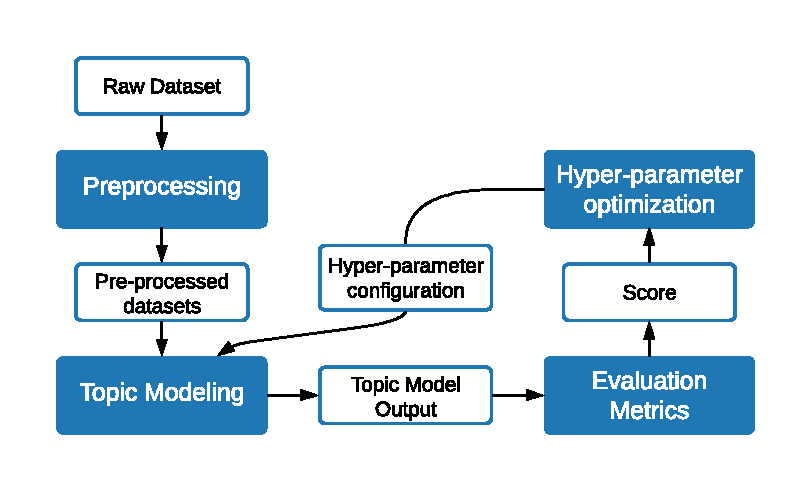
\includegraphics[width=0.7\textwidth]{figures/octis.pdf}
    \caption{Workflow of the OCTIS framework}
    \label{fig:octis}
\end{figure}

OCTIS offers a range of evaluation metrics for assessing topic models, such as coherence, diversity, and classification metrics.

The discovery of good hyper-parameter settings relies on a Bayesian Optimization (BO) approach \cite{archetti_bayesian_2019, galuzzi_hyperparameter_2020, snoek_practical_2012}, where the objective can be any of the available evaluation metrics. Given the potential variability in performance outcomes due to noise, the objective function is defined as the median performance across multiple runs of the model under the same hyperparameter settings for the chosen evaluation metric.

BO is a sequential, model-based optimization technique for noisy black-box functions that are costly and complex to evaluate directly, such as topic models. Its main idea involves using all previously evaluated hyperparameter settings to approximate the performance metric's value, and then selecting new, likely better hyperparameter settings for the next run. The approximation is done by a probabilistic \textit{surrogate model}, which has a prior belief of the objective function based on observed hyperparameter settings. The selection of the next hyperparameter settings is driven by optimizing an \textit{acquisition function}, which uses the uncertainty within the posterior distribution to guide the exploration of the parameter space.

OCTIS is useful for our use case, as it provides a unified framework for training the proposed BERTopic model alongside the baseline models, facilitating their comparison across a variety of evaluation metrics. In fact, in the original BERTopic paper, \citet{grootendorst_bertopic_2022} employed OCTIS to evaluate the model's performance.

Additionally, we can utilize OCTIS' hyperparameter optimization capabilities (BO) to find good hyperparameter settings for the proposed BERTopic model.

\section{Chapter conclusion}
\label{sec:chapter_conclusion_preliminaries}
This chapter provides an overview of topic modeling approaches, from traditional statistical methods to modern embedding-based techniques, along with evaluation metrics for assessing their performance.

While LDA \cite{blei_latent_2001} and NMF \cite{shahnaz_document_2006, kasiviswanathan_emerging_2011, yan_learning_2013} are seminal and widely adopted models that have proven effective across various domains, they are probabilistic, treating words as discrete tokens without considering their semantic relationships. Traditional word embedding techniques like GloVe \cite{pennington_glove_2014} and Word2Vec \cite{mikolov_efficient_2013} attempted to address this by creating context-free embedding spaces, but they still assign a single, static embedding to each word, limiting their ability to capture the nuanced meanings words can have in different contexts \cite{thompson_topic_2020}.

Top2Vec \cite{angelov_top2vec_2020} and BERTopic \cite{grootendorst_bertopic_2022} advance beyond these earlier approaches by leveraging embedding techniques that better capture semantic relationships. These models utilize transformer-based architectures that can understand words in context. Unlike GloVe and Word2Vec, these models can generate contextual embeddings where the same word can have different representations depending on its usage.

BERTopic improves upon Top2Vec's foundation by introducing several innovations. The addition of c-TF-IDF provides a method for identifying distinctive terms within topics, while the optional fine-tuning step allows for refinement of topic representations using language models. These innovations have led to superior performance on standard metrics, with BERTopic achieving higher NPMI (coherence) and diversity scores compared to other approaches \cite{grootendorst_bertopic_2022}. BERTopic's modular architecture, comprising separate components for embeddings, dimensionality reduction, clustering, c-TF-IDF, and topic representation, makes it possible to evolve the model as new embedding models, clustering algorithms, and dimensionality reduction techniques are introduced. 

BERTopic's modular design allows for selecting state-of-the-art components at each processing stage. For embeddings, Salesforce SFR-Embedding-2\_R \cite{noauthor_salesforcesfr-embedding-2_r_2024} is currently one of the best models on the MTEB benchmark \cite{muennighoff_mteb_2023}. In the dimensionality reduction step, UMAP has been shown to better preserve both local and global data characteristics compared to alternatives like PCA and t-SNE \cite{mcinnes_umap_2020}. For clustering, HDBSCAN demonstrates several advantages over conventional algorithms: unlike k-means, it doesn't assume spherical clusters or require pre-specifying the number of topics; and compared to DBSCAN, it adaptively identifies clusters across different density scales, making it more robust for heterogeneous document collections \cite{campello_density-based_2013, allaoui_considerably_2020}.

Although Top2Vec and BERTopic utilize transformer-based embedding models that are expensive to train, they leverage pre-trained versions of these models, eliminating the training overhead and making their practical application comparable in computational cost to traditional approaches.

These reasons make BERTopic particularly well-suited for generating tags for OpenML dataset descriptions. The modular nature of the model also ensures it can evolve alongside advances in language models and embedding techniques, making it a sustainable long-term solution.



It is also important to highlight the state of evaluation metrics in the field. Topic modeling evaluation has largely converged on using NPMI coherence and topic diversity as primary automated metrics \cite{doogan_topic_2021, hoyle_is_2021, mimno_optimizing_nodate, lau_machine_2014}. These metrics are widely adopted in the literature, where researchers typically report coherence and diversity scores alongside human evaluation results.

The widespread adoption of NPMI and diversity metrics influenced our choice to use them as optimization and evaluation metrics. Furthermore, these metrics provide complementary perspectives on topic quality: while coherence measures how semantically related words within a topic are, diversity ensures that topics remain distinct from one another. This creates balance, as increasing coherence often leads to less diverse topics (since semantically related words are often similar), while maximizing diversity might reduce coherence. This balance helps prevent the model from repeatedly selecting the same high-frequency terms across different topics.

However, we acknowledge the limitations of these automated metrics. Several studies have found that coherence and diversity scores show only small to moderate correlations with human judgment \cite{doogan_topic_2021, hoyle_is_2021}. The relationship between these metrics and actual topic quality, as perceived by humans, is not straightforward. Some researchers have questioned whether automated topic model evaluation is fundamentally flawed \cite{hoyle_is_2021}, pointing out that coherence metrics may not capture the nuanced ways humans interpret and understand topics.

While other evaluation metrics exist, such as perplexity and various classification-based metrics, they are less commonly adopted in the field and their relationship with human judgment is even less studied. Additionally, many of these metrics are not applicable to modern neural topic models \cite{doogan_topic_2021}, which often generate terms not present in the original corpus through fine-tuning steps.

For implementing these metrics and comparing different topic models, we choose to use the OCTIS framework \cite{terragni_octis_2021}. OCTIS provides a standardized environment for training and evaluating topic models, ensuring fair comparisons between different approaches. Its support for Bayesian optimization of hyperparameters is particularly valuable for our work with BERTopic, as it allows us to explore the hyperparameter space while optimizing for both coherence and diversity.

Given the limitations of automated metrics, we acknowledge that they should not be the sole basis for evaluating topic model performance. While we use these metrics for optimization and baseline comparisons to align with field practices, we place greater emphasis on human evaluation, which will be discussed in later chapters. This approach allows us to more directly assess whether the generated topics and tags are truly meaningful to users, which is ultimately the most important criterion for a practical topic modeling system.

This chapter primarily addresses \hyperref[rq2]{\textbf{RQ2}} and \hyperref[rq3]{\textbf{RQ3}}. For \hyperref[rq2]{\textbf{RQ2}}, we conduct an examination of topic modeling approaches, from traditional statistical methods such as LDA and NMF to modern embedding-based techniques like Top2Vec and BERTopic. We analyze their advantages and disadvantages, particularly focusing on BERTopic's modularity and ability to evolve with advances in the field. For \hyperref[rq3]{\textbf{RQ3}}, we investigate evaluation metrics, explaining why NPMI coherence and diversity have become standard metrics in the field while acknowledging their limitations. We also introduce OCTIS as our framework for implementing these metrics and optimizing model performance.